\chapter{Gauß-Layout-System}\label{chap:gausspage}

Dieses Kapitel beschreibt das allgemeine Layoutsystem zur Erstellung von
Inhalten und Hintergründen im Gaußraster des Corporate Designs.
Es findet als Basis unter anderem bei der Darstellung von Titelseiten oder
Veranstaltungspostern Anwendung. Die hier beschriebenen Befehle und Optionen
können daher in weiten Teilen auf alle Konstrukte in \tubslatex angewendet
werden, die im Gauß-Layout dargestellt werden.

Es gibt grundlegend drei verschiedene Möglichkeiten das Gauß-Layout-System
zu nutzen:
\begin{itemize}
  \item Definition einer Hintergrunddarstellung,
  \item Verwendung von Textboxen,
  \item Kombination von Hintergrundelementen und Textboxen,
\end{itemize}
wobei die Letztgenannte den Regelfall darstellt.

\section{Hintergrund-Layout}\label{sec:gausspage:bglayout}

\begin{Declaration}
  \Macro{bglayout}\OParameter{Optionen}\Parameter{Layout}
\end{Declaration}

Mit Hilfe des Befehls \Macro{bglayout} kann das Hintergrundlayout im Gaußraster gesetzt werden.
% Dies hat in etwa dieselbe Funktionalität wie vorbedrucktes Papier.
Alle Komponenten werden im Hintergrund und unabhängig vom Inhalt der Seite
dargestellt.

Folgende \PName{Optionen} können gewählt werden:

\begin{Declaration}
  \KOption{sender}\PName{top/bottom}
\end{Declaration}

Steuert die Positionierung des Absenderbereiches.
Der Wert \PValue{top} platziert den Absenderbereich am oberen,
der Wert \PValue{bottom} am unteren Ende des Blattes.

\begin{Declaration}
  \KOption{pages}\PName{all/single}
\end{Declaration}

Legt fest für welche Seiten die aktuelle Einstellung gelten soll.
Der Wert \PValue{all} besagt, dass es für alle folgenden Seiten gelten soll,
während mit \PValue{single} die Darstellung nur auf der aktuellen Seite geändert 
wird.

\begin{Declaration}
  \Option{designhelper}
\end{Declaration}

Darstellung der verfügbaren Segmente und Logo-Positionen durch schwarze Rahmen, abhängig von der Platzierung des Absenderbereiches.
Diese Option ist hilfreich für das Design einer Seite im Gauß-Layout.


\subsection{Elemente}\label{subsec:gausspage:bgelement}

\begin{Declaration}
  \Macro{bgelement}\OParameter{Darstellung}\PParameter{Höhe}
\end{Declaration}

Erstellt ein Hintergrundelement im Gaußraster mit angegebener \PName{Höhe}.
Diese gibt an wieviele Segmente des Gauß-Layouts für das aktuelle Element
verwendet werden sollen.
Die Segmente werden dabei von oben nach unten Belegt.
Abhängig von der Position des Absenderbereiches werden die Segmente
entweder nach unten kleiner (Absender oben) oder größer (Absender unten).

\noindent\begin{minipage}{0.4\textwidth}
Pro Seite stehen allgemein maximal 8 (Hochformat) bzw. 6 (Querformat)
Segmente zur Verfügung. Werden mehr belegt, so kommt es zu einer Fehlermeldung.
\end{minipage}
\begin{minipage}{0.6\textwidth}\centering
\begin{minipage}[b]{0.4\textwidth}\centering
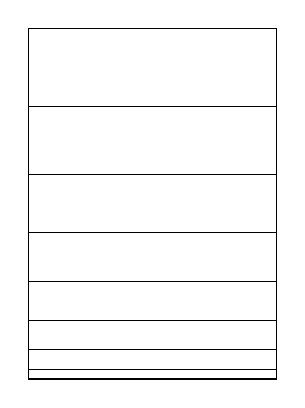
\begin{tikzpicture}[scale=1.5]
  \def\tikzpageheight{2.97}
  \def\tikzpagewidth{2.1}
  \draw (0,0) rectangle (\tikzpagewidth, \tikzpageheight);
  \foreach \i in {1,3,6,10,15,21,28}{%
    \draw (0, \i*\tikzpageheight/36) -- (\tikzpagewidth, \i*\tikzpageheight/36);
  }
\end{tikzpicture}\\
Hochformat\\ (8 Segmente)
\end{minipage}
\begin{minipage}[b]{0.45\textwidth}\centering
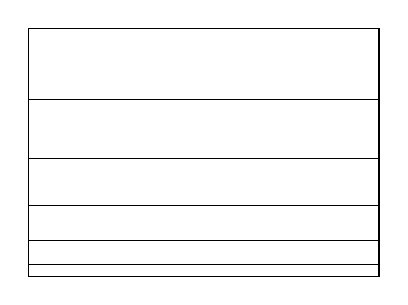
\begin{tikzpicture}[scale=1.5]
  \def\tikzpageheight{2.1}
  \def\tikzpagewidth{2.97}
  \draw (0,0) rectangle (\tikzpagewidth, \tikzpageheight);
  \foreach \i in {1,3,6,10,15}{%
    \draw (0, \i*\tikzpageheight/21) -- (\tikzpagewidth, \i*\tikzpageheight/21);
  }
\end{tikzpicture}\\
Querformat\\ (6 Segmente)
\end{minipage}
\end{minipage}
\vspace*{0pt}


Der optionale Parameter \PName{Darstellung} kann die folgenden Einstellungen verarbeiten:


\begin{Declaration}
  \KOption{bgcolor}\PName{Farbe}\\
  \KOption{bgimage}\PName{Bild-Datei}\\
  \KOption{imagefit}\PName{Darstellungsoption}
\end{Declaration}

Mit \OptionValue{bgcolor}{Farbe} wird das Hintergrundelement mit der angegebenen
Farbe gefüllt. Die verfügbaren Farben können Kapitel~\ref{chap:tubscolors}
entnommen werden.

Die Option \OptionValue{bgimage}{Bild-Datei} erlaubt dagegen die Darstellung
eines Hintergrundbildes im Element.
Da der Darstellungsbereich fest vorgegeben ist, muss das eingebundene Bild
in diesen Bereich eingepasst werden. Dies geschieht automatisch, die Art
der Einpassung lässt sich aber mit der Option \Option{imagefit} kontrollieren.
Sie erlaubt folgende Einstellungen:


\begin{desctable}
\entry{\PValue{clipped}}{%
  Automatisches randloses Zuschneiden. Dies ist die Standardeinstellung.
  Wählt abhängig von Seitenverhälntissen automatisch zwischen
  \PValue{clipx} und \PValue{clipy}.
}
\entry{\PValue{clipx}/\PValue{fitheight}}{%
  Vertikale Skalierung, horizontaler Zuschnitt.
  Je nach Seitenverhälntissen von Bild und Darstellungsbereich können
  Teile des Bildes weggeschnitten werden.
}
\entry{\PValue{clipy}/\PValue{fitwidth}}{%
  Horizontale Skalierung, vertikaler Zuschnitt
  Je nach Seitenverhälntissen von Bild und Darstellungsbereich können
  Teile des Bildes weggeschnitten werden.
}
\entry{\PValue{scaled}}{%
  Horizontale \emph{und} vertikale Skalierung.
  Es wird kein Teil des Bildes abgeschnitten.
  Dabei kann jedoch das Seitenverhältnis stark verändert und somit 
  das Bild verzerrt werden.
}
\end{desctable}
% TODO: table label?

\begin{Declaration}
  \Macro{showtubslogo}\OParameter{Optionen}
\end{Declaration}

Bewirkt Darstellung des TU-Siegelbandlogos im aktiven Layout.
Die \PName{Optionen} erlauben unter anderem die Angabe der Darstellungsseite
(links/rechts).

\begin{Declaration}
  \Option{links}/\Option{inside}\\
  \Option{rechts}/\Option{outside}
\end{Declaration}

Mit der Logo-Option \Option{links} bzw. \Option{inside} wird das Logo auf der Seite
links bzw. innen dargestellt. Dies ist die Standardeinstellung.
Mit der Option \Option{rechts} bzw. \Option{outside} wird das Logo auf der
Seite rechts bzw. außen dargestellt.

\begin{Declaration}
  \Option{plain}
\end{Declaration}

Die Logo-Option \Option{plain} bewirkt, dass nicht das Logo selber,
sondern stattdessen eine gleichgroße einfarbige Fläche in der Farbe
des Siegelbandlogos dargestellt wird.
Dies ist vor allem für Rückseiten sinnvoll.


\begin{Declaration}
  \Macro{showlogo}\PParameter{Logo}
\end{Declaration}

Bewirkt Darstellung eines Individuellen Logos im aktuellen Layout.
\PName{Logo} kann dabei entweder einfacher Text oder auch ein 
mit \Macro{includegraphics} eingebundenes Bild sein.
In diesem Fall wird eine Eingebundene Grafik automatisch auf die korrekte
Höhe skaliert (solange in den Optionen nicht anders angegeben).

Die Positionierung wird automatisch an die Position des Absenderbereichs und
die Positionierung des Siegelbandlogos angepasst.
Wird dies links bzw. innen platziert, so steht das individuelle
Logo rechts bzw. außen.

\begin{Declaration}
  \Macro{showtopline}
\end{Declaration}

Bewirkt Darstellung einer Trennlinie zwischen Absender und Kommunikationsbereich
im aktuellen Layout.

\begin{lstlisting}[captionpos=b,caption={Beispiel-Nutzung von bglayout}]
\bglayout[pages=single]{%
  \showtubslogo
  \bgelement[bgimage=mypic.jpg]{2}
  \bgelement[bgcolor=tuGreen]{3}
  \bgelement[bgcolor=tuGreenDark]{3}
}
\end{lstlisting}


\section{Text-Boxen}

\begin{Declaration}
  \XMacro{begin}\PParameter{\Environment{gaussbox}}%
          \OParameter{Optionen}%
          \Parameter{hPos}%
          \Parameter{vPos}%
          \Parameter{Breite}%
          \Parameter{Höhe}\\
  \quad\dots\\
  \XMacro{end}\PParameter{gaussbox}
\end{Declaration}

Mit \Environment{gaussbox} können einfache Boxen im Gaußraster gesetzt werden,
die unabhängig vom Seiteninhalt an der festgelegten Position gesetzt werden.
Neben der vertikalen Größe kann auch eine vertikale Größe im Spaltenraster
definiert werden, also mit einer Unterteilung in 6 Spalten.

Der Wert \PName{vPos} gibt dabei das Start-Segment im Gaußraster an
($[1\ldots 8]$ bzw. $[1\ldots6]$),
der Wert \PName{hPos} die Start-Spalte ($[1\ldots6]$).
Mit \PName{Höhe} wird angegeben wieviele Gauß-Segmente die Box umfassen soll,
mit \PName{Breite} wieviel Spalten.

\begin{Example}
  \begin{lstlisting}
\begin{gaussbox}{1}{1}{3}{2}
  // Inhalt
\end{gaussbox}
  \end{lstlisting}
  Erzeugt eine Text-Box, die halbe Text-Breite aufweist und vom oberen
  Rand aus in der Höhe 2 Segmente einnimmt.
\end{Example}


\section{Kombination}

Die hier vorgestellte Kombination ist für die einfache Erstellung ganzer Seiten
inklusive Text im Gauß-Raster gedacht.
Sie bildet auch die Basis für die Umgebungen von Veranstaltungspostern und
für Titelseiten von Dokumenten.

\begin{Declaration}
  \XMacro{begin}\PParameter{\Environment{gausspage}}%
    \OParameter{Optionen}\\
  \quad\dots\\
  \XMacro{end}\PParameter{gausspage}
\end{Declaration}

Die Umgebung \Environment{gausspage} kombiniert das Hintergrund-Layout
und die Textboxen zu einem Interface, das dem Standard-Anwendungsfall für
das Gauß-Layout gerecht wird, da Textboxen und Hintergrund im Regelfall
genau gleich positioniert sind.

Als \PName{Optionen} können alle in Kapitel~\ref{sec:gausspage:bglayout}
für \Macro{bglayout} definierten Optionen verwendet werden.
Die Option \Option{pages} ist standardmäßig auf \PValue{single}
eingestellt.% TODO: check

\begin{Declaration}
  \XMacro{begin}\PParameter{\Environment{segment}}%
    \OParameter{Optionen}
    \Parameter{Höhe}\\
  \quad\dots\\
  \XMacro{end}\PParameter{segment}
\end{Declaration}

Mit der Umgebung \Environment{segment} könnnen die einzelnen
Segmente gesetzt werden.
Diese gehen jeweils über die ganze Textbreite und orientieren sich
in der vertikalen Positionierung am Interface von \Macro{bgelement}.
Die \PName{Höhe} gibt also die Anzahl der verwendete Basis-Segmente an
und belegt diese von oben nach unten.

Als \PName{Optionen} können alle in Kapitel~\ref{subsec:gausspage:bgelement}
für \Macro{bgelement} definierten Optionen verwendet werden. % TODO: check


\begin{lstlisting}[captionpos=b,caption={Beispiel-Nutzung von gausspage}]
\begin{gausspage}{%
  \showtubslogo
  \begin{segment}[bgimage=mypic.jpg]{2}
    // Inhalt
  \end{segment}
  \begin{segment}[bgcolor=tuGreen]{3}
    // Inhalt
  \end{segment}
  \begin{segment}[bgcolor=tuGreenDark]{3}
    // Inhalt
  \end{segment}
}
\end{lstlisting}

% TODO: place? ref?
\begin{figure}\centering
  \fboxsep0mm
  \begin{minipage}{0.35\textwidth}
    \fbox{\includegraphics[width=\textwidth,page=1]{examples/gausssegments.pdf}}
    \subcaption{Absenderbereicht oben}\label{fig:gausspage:topsender}
  \end{minipage}
  \quad
  \begin{minipage}{0.35\textwidth}
    \fbox{\includegraphics[width=\textwidth,page=2]{examples/gausssegments.pdf}}
    \subcaption{Absenderbereicht unten}\label{fig:gausspage:bottomsender}
  \end{minipage}
  \caption{Gaußraster mit möglichen Logo-Positionen}\label{fig:gausspage}
\end{figure}
